\documentclass[12pt]{extarticle}
\usepackage{phys440}

\title{PHYS440 - Project: HHL Algorithm}
\author{John Hurst}
\date{June 2024}

\begin{document}
\maketitle

%%%%%%%%%%%%%%%%%%%%%%%%%%%%%%%%%%%%%%%%%%%%%%%%%%%%%%%%%%%%%%%%%%%%%%%%%%%%%%%%%%%%%%%%%%%%%%%%%%%%
\section{Introduction}

The HHL algorithm for solving linear systems\cite{hhl2009} is one of the first algorithms to promise a quantum speedup for a variety of real-world problems.
The walk-through in \cite{zaman2023step} shows the mathematics for each step and provides background on the relevant quantum computing concepts.
The paper gives a numerical example to illustrate the steps, and provides MATLAB and Qiskit code for the example.

For my PHYS440 project I studied the walkthrough to understand the HHL algorithm in some detail,
and supplemented this by reading several other introductory sources such as \cite{baaquie2023} and \cite{hidary2021}.

I ported the MATLAB sample code to two different Mathematica implementations.
The first implementation is a direct port of the matrix formulation of the circuit from MATLAB.
The second implementation uses the Wolfram Quantum Framework to implement the example using the QuantumCircuitOperator feature.

The paper's example uses a 2x2 matrix, and only two clock qubits, which does not sufficiently illustrate some features of the algorithm.
I created my own example with a 4x4 matrix and three clock qubits, to study these features in more detail.

I then followed up with some more reading on the limits and applicability of HHL, starting from Aaronson's well-known paper \cite{aaronson2015read}.

The remainder of this report is in two parts.
Part \ref{sec:implementation} discusses implementation details of the more general numerical example, in particular the handling of the ancilla rotation.
Part \ref{sec:applications} discusses the applicability of the HHL algorithm to real-world problems.

\section{Implementation Notes}\label{sec:implementation}

This report will not repeat all the details from \cite{zaman2023step}.
I will focus instead on what I found by generalising the example to a larger matrix and number of clock qubits.

My HHL circuit for a 4x4 matrix and three clock qubits is shown in Figures \ref{fig:circuit1}-\ref{fig:circuit3}.
The first register, labelled $b$, with two qubits, begins with the input state, and carries the result $x$ at the end.
The second register, labelled $q$, with three qubits, is the clock register.
The third register, labelled $a$, with one qubit, is the ancilla register.

Figure \ref{fig:circuit1} shows the state preparation and QPE.
Because the goal of my implementation is to understand the algorithm,
not to provide a practical implementation, I have provided the input state directly in Mathematica using the \texttt{QuantumTensorProduct[]} function:
\begin{lstlisting}[language=Mathematica]
psi1 =
    QuantumTensorProduct[
        Join[{QuantumState[Normalize[b]]},
              ConstantArray[QuantumState[{1, 0}], n + 1]]]
\end{lstlisting}
\begin{figure}[h]
\centering
$\begin{array}{c}
\Qcircuit @C=.5em @R=.8em {
\lstick{a}   & \qw & \qw      & \qw       & \qw & \qw & \qw & \qw & \qw & \qw & \qw & \qw & \qw & \qw & \qw \\
& & & & & & & \mbox{IQFT} & & & & & & & \\
\lstick{q_0} & \qw & \gate{H} & \ctrl{3} & \qw & \qw & \qswap & \gate{H} & \ctrl{1} & \qw & \ctrl{2} & \qw & \qw & \qw & \qw \\
\lstick{q_1} & \qw & \gate{H} & \qw & \ctrl{2} & \qw & \qw & \qw & \gate{R_{-1/2}} & \gate{H} & \qw & \ctrl{1} & \qw & \qw & \qw \\
\lstick{q_2} & \qw & \gate{H} & \qw & \qw & \ctrl{1} & \qswap \qwx[-2] & \qw & \qw & \qw & \gate{R_{-1/4}} & \gate{R_{-1/2}} & \gate{H} & \qw & \qw \\
\lstick{b_0} & \multigate{1}{\text{prepare } b} & \qw & \multigate{1}{U} & \multigate{1}{U^2} & \multigate{1}{U^4} & \qw & \qw & \qw & \qw & \qw & \qw & \qw & \qw & \qw \\
\lstick{b_1} & \ghost{\text{prepare } b} & \qw & \ghost{U} & \ghost{U^2} & \ghost{U^4} & \qw & \qw & \qw & \qw & \qw & \qw & \qw & \qw & \qw
\gategroup{2}{7}{5}{13}{1.4em}{--}
}
\end{array}$
\caption{State preparation and QPE}
\label{fig:circuit1}
\end{figure}
In real world applications, state preparation is a nontrivial problem, as discussed in \cite{aaronson2015read} and \cite{hhl2009}.

This part of the circuit is conceptually the same as in \cite{zaman2023step},
but because there are four values in the input $b$ and four unknowns in $x$, the unitary operation in the QPE has two target qubits instead of one.
Also, because there are three clock qubits, in QPE we apply $U$, $U^2$ and $U^4$, and the IQFT subcomponent is extended to three qubits.

Figure \ref{fig:circuit2} shows the ancilla rotation.
\begin{figure}[h]
\centering
$\begin{array}{c}
\Qcircuit @C=.5em @R=.8em {
\lstick{a}   & \qw & \gate{RY(\theta_1=2\inv{\sin}\frac{1}{4})} & \gate{RY(\theta_2=2\inv{\sin}\frac{1}{3})} & \gate{RY(\theta_3=\frac{\pi}{3})} & \gate{RY(\theta_4=\pi)} & \qw \\
\lstick{q_0} & \qw & \ctrlo{-1} & \ctrl{-1}  & \ctrlo{-1} & \ctrl{-1}  & \qw \\
\lstick{q_1} & \qw & \ctrlo{-2} & \ctrl{-2}  & \ctrl{-2}  & \ctrlo{-2} & \qw \\
\lstick{q_2} & \qw & \ctrl{-3}  & \ctrlo{-3} & \ctrlo{-3} & \ctrlo{-3} & \qw \\
% \lstick{b_0} & \qw & \qw & \qw & \qw & \qw & \qw \\
% \lstick{b_1} & \qw & \qw & \qw & \qw & \qw & \qw \\
}
\end{array}$
\caption{Ancilla rotation}
\label{fig:circuit2}
\end{figure}

This part of the circuit is the most interesting part of the project.

As discussed in class, I was confused about the number of rotations on the ancilla qubit.
In \cite{zaman2023step} there are two rotations on the ancilla qubit, using angles $\theta_1$ and $\theta_2$, and controlled by the two clock qubits.
The angles $\theta_1$ and $\theta_2$ are calculated from the eigenvalues of the matrix $A$.
So it was unclear to me whether there should be a distinct rotation were per eigenvalue, or per clock qubit.
It seemed to me from the construction of the circuit that it must be a rotation per clock qubit.
And also, in real-world applications we might have billions of unknowns and eigenvalues, but we will always have a fairly limited number of clock qubits, determined by the precision desired.
So it seemed to me that it would not be practical to consider rotations per eigenvalue.

It turns out that my thinking was not correct.
The rotations on the ancilla qubit achieve the inversion of the eigenvalues,
and so to get a solution with perfect accuracy it is necessary to have a rotation per eigenvalue.
However, in real world implementations, it's unlikely this would actually be done for large numbers of input qubits.
By being selective and careful about the rotations, an approximate solution satisfies the accuracy bounds in \cite{hhl2009}.
A recent paper, \cite{morgan2024enhanced}, discusses filtering rotations ``by relevance'' to maintain circuit depth advantages.

In the circuit in Figure \ref{fig:circuit2}, I have implemented four rotations with angles $\theta_1$, $\theta_2$, $\theta_3$ and $\theta_4$,
which correspond precisely to the eigenvalues $\lambda_1$, $\lambda_2$, $\lambda_3$ and $\lambda_4$ of the matrix $A$.
They are controlled by the clock qubits according to the binary representation of the eigenvalue phases on the clock qubits.
So for example, the first eigenvalue is $\lambda_1=\frac{4}{3}$.
In the Hamiltonian $e^{i\Lambda t}$ this eigenvalue has corresponding value $e^{i\lambda_1t}=e^{i\frac{4}{3}\times\frac{3\pi}{4}}=e^{2\pi i \frac{1}{2}}$.
Therefore the phase for this eigenvalue is $\phi_1=\frac{1}{2}$, which in binary is 0.100b.
Therefore the rotation for this eigenvalue should occur when qubit $q_2$ is set and qubits $q_1$ and $q_0$ are not set.
The rotation angle is obtained via the formula from \cite{zaman2023step}: $\theta_1=2\inv{\sin}\bar{\lambda}_1$,
where $\bar{\lambda}_1$ is the eigenvalue scaled by a factor that makes all the eigenvalues integers:
\[
\bar{\lambda_j}=\frac{2^n\lambda_jt}{2\pi}
\]
In this way we obtain the phases, controlling qubits, and rotation angles for all the eigenvalues, shown in the table below:
\begin{center}
\begin{tabular}{|c|c|c|c|c|}
\hline
Eigenvalue & $e^{i\lambda t}=e^{2\pi i\phi}$ & Phase & Qubits & Angle \\
\hline
$\lambda_1=\frac{4}{3}$ & $e^{i\lambda_1t}=e^{i \frac{4}{3} \times \frac{3\pi}{4}}=e^{2\pi i \frac{1}{2}}$ & $\phi_1=\frac{1}{2}=$0.100b & $q_2\overline{q_1}\overline{q_0}$ & $\theta_1=2\inv{\sin}\frac{1}{4}$ \\
$\lambda_2=1$           & $e^{i\lambda_2t}=e^{i 1 \times \frac{3\pi}{4}}=e^{2\pi i \frac{3}{8}}$   & $\phi_2=\frac{3}{8}=$0.011b & $\overline{q_2}q_1q_0$ & $\theta_2=2\inv{\sin}\frac{1}{3}$ \\
$\lambda_3=\frac{2}{3}$ & $e^{i\lambda_3t}=e^{i \frac{2}{3} \times \frac{3\pi}{4}}=e^{2\pi i \frac{1}{4}}$ & $\phi_3=\frac{1}{4}=$0.010b & $\overline{q_2}q_1\overline{q_0}$ & $\theta_3=2=2\inv{\sin}\frac{1}{2}=\frac{\pi}{3}$ \\
$\lambda_4=\frac{1}{3}$ & $e^{i\lambda_4t}=e^{i \frac{1}{3} \times \frac{3\pi}{4}}=e^{2\pi i \frac{1}{8}}$ & $\phi_4=\frac{1}{8}=$0.001b & $\overline{q_2}\overline{q_1}q_0$ & $\theta_4=2=2\inv{\sin}\frac{1}{1}=\pi$ \\
\hline
\end{tabular}
\end{center}
The controlling qubits and rotation angles correspond to the circuit portion in Figure \ref{fig:circuit2}.
% TODO: How might this have been shown more clearly in zaman2023step?

Figure \ref{fig:circuit3} shows the reverse QPE and measurement.
As in \cite{zaman2023step}, if the ancilla qubit is measured in state $\ket{1}$,
then the $b$ register holds the correct $x$ result.
If the ancilla qubit is measured in state $\ket{0}$, the result is discarded and the circuit must be run again.
\begin{figure}[h]
\centering
$\begin{array}{c}
\Qcircuit @C=.4em @R=.7em {
    \lstick{a}   & \qw & \qw & \qw & \qw & \qw & \qw & \qw & \qw & \qw & \qw & \qw & \qw & \meter \\
    & & & \mbox{QFT} & & & & & & & & & & & & \\
    \lstick{q_2} & \qw & \qw & \qw & \ctrl{2} & \qw & \ctrl{1} & \gate{H} & \qswap & \qw & \qw & \ctrl{3} & \gate{H} & \qw \\
    \lstick{q_1} & \qw & \qw & \ctrl{1} & \qw & \gate{H} & \gate{R_{1/2}} & \qw & \qw & \qw & \ctrl{2} & \qw & \gate{H} & \qw \\
    \lstick{q_0} & \qw & \gate{H} & \gate{R_{1/2}} & \gate{R_{1/4}} & \qw & \qw & \qw & \qswap \qwx[-2] & \ctrl{1} & \qw & \qw & \gate{H} & \qw \\
\lstick{b_0} & \qw & \qw & \qw & \qw & \qw & \qw & \qw & \qw & \multigate{1}{U^{-4}} & \multigate{1}{U^{-2}} & \multigate{1}{U^{-1}} & \qw & \meter \\
\lstick{b_1} & \qw & \qw & \qw & \qw & \qw & \qw & \qw & \qw & \ghost{U^{-4}} & \ghost{U^{-2}} & \ghost{U^{-1}} & \qw & \meter
\gategroup{2}{3}{5}{8}{1.4em}{--}
}
\end{array}$
\caption{Inverse QPE and measurement}
\label{fig:circuit3}
\end{figure}

\begin{figure}[H]
\centering
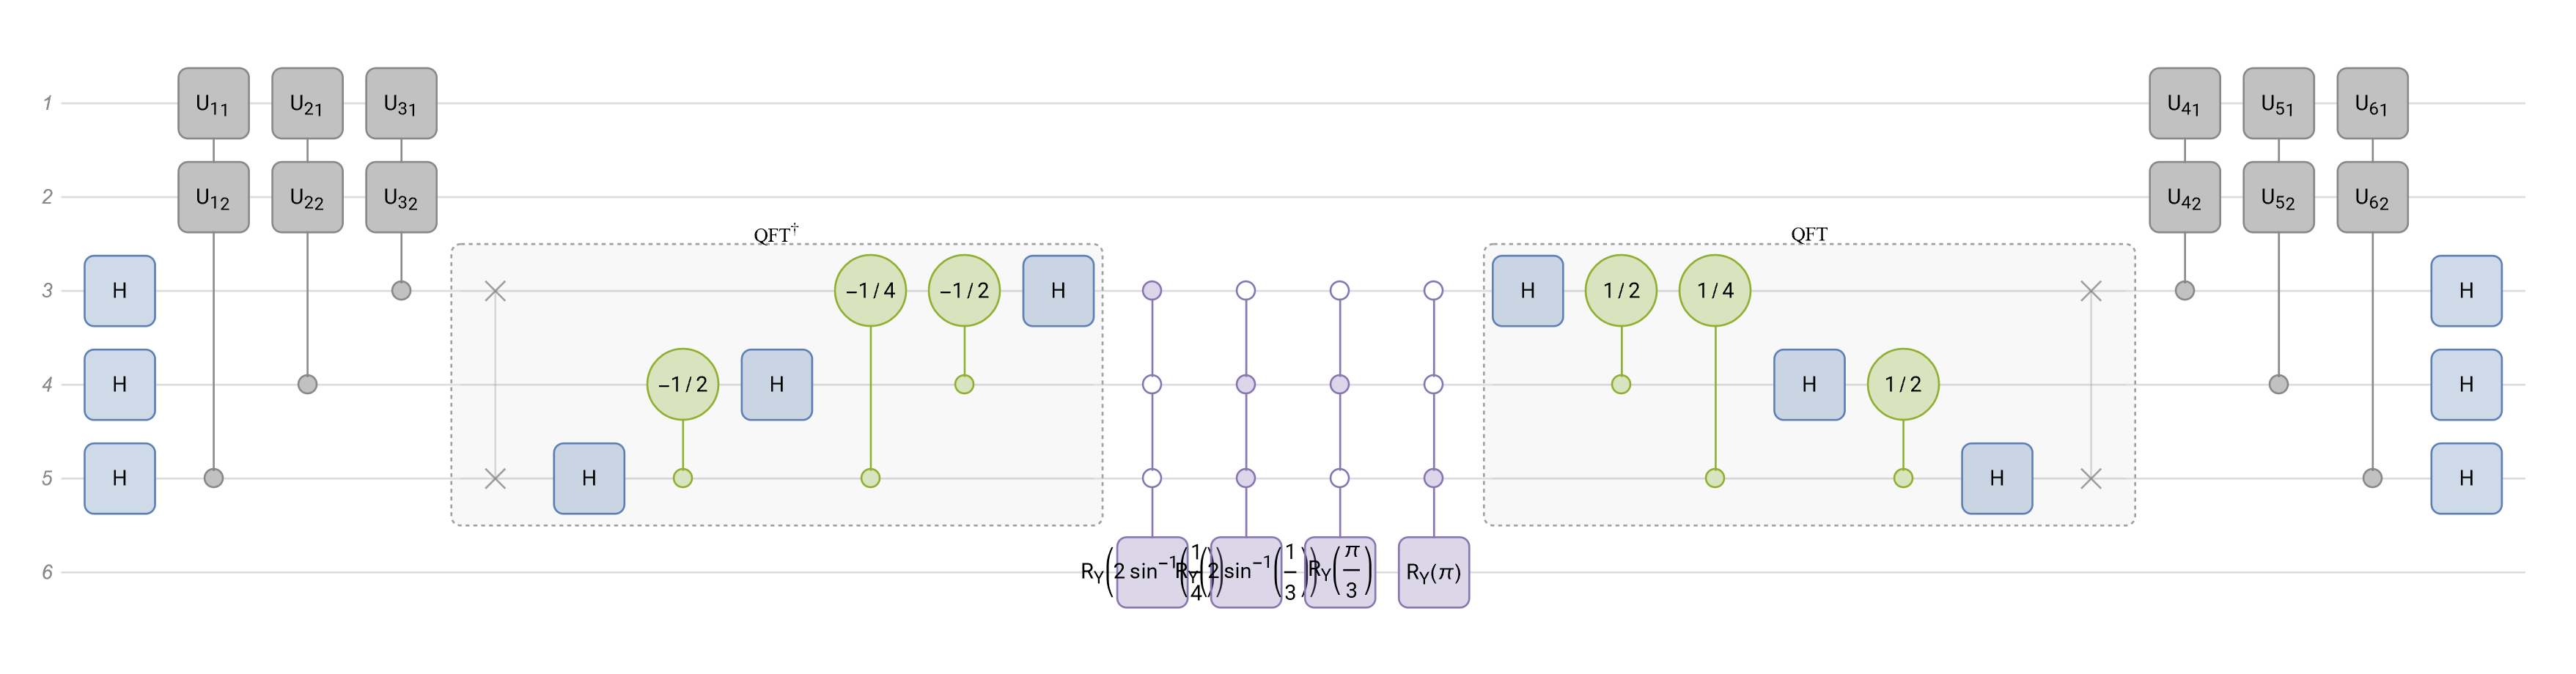
\includegraphics[width=0.80\textwidth]{images/project_hhl_4x4_mathematica.png}
\caption{Mathematica circuit for 4x4 problem}
\label{fig:hhl_4x4_mathematica}
\end{figure}

\begin{figure}[H]
\centering
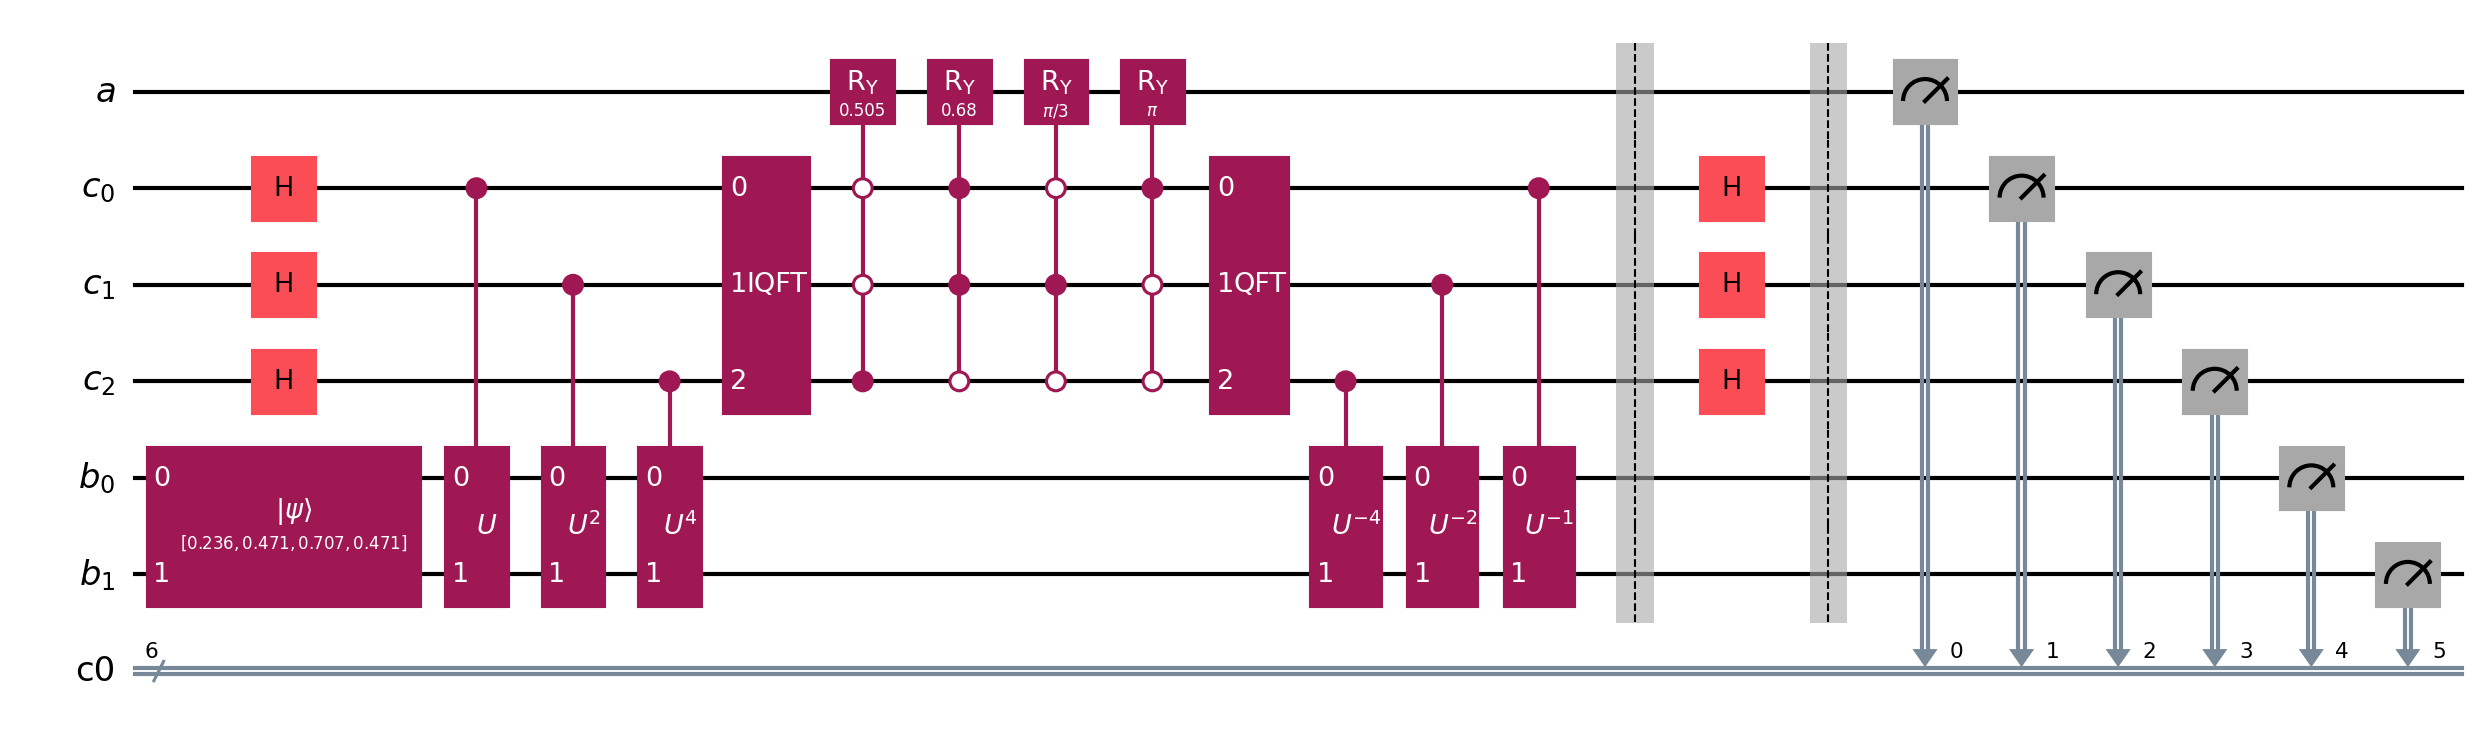
\includegraphics[width=0.80\textwidth]{images/project_hhl_4x4.png}
\caption{Qiskit circuit for 4x4 problem}
\label{fig:hhl_4x4_qiskit}
\end{figure}


% TODO: Figure for Qiskit circuit

% 000000  45393
% 000001  138971  0.1529  0.1977
% 010000  84
% 010001  204263  0.2247  0.2397
% 100000  45357
% 100001  324365  0.3568  0.3020
% 110000  84
% 110001  241483  0.2656  0.2606
% Prob(ancilla |0⟩) = 0.9091

\section{Applications}\label{sec:applications}

\printbibliography
\addcontentsline{toc}{section}{References}


\end{document}
